\documentclass[11pt,twoside,a4paper]{article}
\usepackage{amsmath}
\usepackage{amssymb}
\usepackage{geometry}
\usepackage{multicol}% multi colomn
\usepackage{graphicx}
\usepackage{float}
\geometry{a4paper,left=2cm,right=2cm,top=1cm,bottom=2cm}
\DeclareMathSizes{12}{20}{14}{10}
\begin{document}
\title{Ex7 186 Fall}
\author{Assignment group 10}
\date{}
\maketitle
\section{Ex. 7.1}
\subsection{Ex. 7.1.1 Hölder's Inequality}
\textbf{Lemma: }
\newline
$\forall a,b\geq 0$, $p>1$ and $\frac{1}{p}+\frac{1}{q}=1$, $ab\leq\frac{a^{p}}{p}+\frac{b^{q}}{q}$.
\newline
Proof: From (1), which is a special case of \textit{Jensen's Inequality}, given in Assignment 6, we have:
$$(a^{p})^{\frac{1}{p}}\cdot (b^{q})^{\frac{1}{q}}=a\cdot b\leq \frac{a^{p}}{p}+\frac{b^{q}}{q}$$
\rightline{Q.E.D.}
\newline
\textbf{Proof of Hölder's Inequality:}
\newline
Let $a_{i}=\frac{|x_{i}|}{||x_{i}||_{p}}$ and $b_{i}=\frac{|y_{i}|}{||y_{i}||_{p}}$, in which $i$=1,2,3,4$\ldots$n.
\newline
From Young's Inequality, we have:
$$a_{i}b_{i}\leq\frac{|x_{i}|^{p}}{p||x_{i}||^{p}_{p}}+\frac{|y_{i}|^{q}}{q||y_{i}||^{q}_{q}}$$
So,$$\sum_{i=1}^{n} a_{i}b_{i}\leq\frac{1}{p}\sum_{i=1}^{n}\frac{|x_{i}|^{p}}{||x_{i}||^{p}_{p}}+\frac{1}{q}\sum_{i=1}^{n}\frac{|y_{i}|^{q}}{||y_{i}||^{q}_{q}}=\frac{1}{p}+\frac{1}{q}=1
$$\rightline{Q.E.D.}
\subsection{Ex. 7.1.2 Minkowski's Ineqality}
Using \textit{Hölder's Inequality} as a lemma.\newline
\textbf{Proof of Minkowski's Inequality: }\begin{align*}
\sum_{j=1}^{n} |x_j + y_j|^p &= \sum_{j=1}^{n} |x_j + y_j||x_j + y_j|^{p-1}\\
&\leq\sum_{j=1}^{n} (|x_j|+|y_j|)|x_j + y_j|^{p-1}\\
&=\sum_{j+1}^{n} |x_j||x_j +y_j|^{p-1}+\sum_{j+1}^{n} |y_j||x_j +y_j|^{p-1}\\
&\leq (\sum_{j=1}^{n} |x_j|^p)^{\frac{1}{p}}\cdot (\sum_{j=1}^{n} |x_j +y_j|^{(p-1)q})^{\frac{1}{q}}+(\sum_{j=1}^{n} |y_j|^p)^{\frac{1}{p}}\cdot (\sum_{j=1}^{n} |x_j +y_j|^{(p-1)q})^{\frac{1}{q}}\\
&=(\sum_{j=1}^{n} |x_j +y_j|^{p})^{\frac{1}{q}}\cdot [(\sum_{j=1}^{n} |x_j|^p)^{\frac{1}{p}}+(\sum_{j=1}^{n} |y_j|^p)^{\frac{1}{p}}]
\end{align*}
Thus, $$\frac{\sum_{j=1}^{n} |x_j + y_j|^p}{\sum_{j=1}^{n} |x_j +y_j|^{p})^{\frac{1}{q}}}=(\sum_{j=1}^{n} |x_j + y_j|^p)^{\frac{1}{p}}\leq [(\sum_{j=1}^{n} |x_j|^p)^{\frac{1}{p}}+(\sum_{j=1}^{n} |y_j|^p)^{\frac{1}{p}}]$$for $\forall p\geq 1$, $q\neq 0$.\newline
\rightline{Q.E.D.}
\subsection{Ex. 7.1.3}
First, for $\forall x\in \mathbb{R}^n$, $||x||_p \geq 0$ and $||x||_p =0$ if and only if $x_1 = x_2 = x_3 = \cdots =x_n =0$.\newline
Besides,\begin{align*}
||x\cdot y||_p &=(\sum_{1\leq i,j\leq n} |x_j \cdot y_j |^p )^{\frac{1}{p}}=({\sum_{i=1}^{n} |x_i |^p}\cdot{\sum_{j=1}^{n} |y_j |^p})^{\frac{1}{p}}\\&=||x||_p \cdot ||y||_p\, .
\end{align*}
Finally,\begin{align*}
||x+y||_p &= (\sum_{j=1}^{n} |x_j + y_j|^p)^{\frac{1}{p}}\leq (\sum_{j=1}^{n} |x_j|^p)^{\frac{1}{p}}+(\sum_{j=1}^{n} |y_j|^p)^{\frac{1}{p}}\\&=||x||_p +||y||_p\, .
\end{align*}
So, $||\cdot||_p$ defines a norm on $\mathbb{R}^n$ for $\forall p\in\mathbb{N}\backslash\{0\}$.
\subsection{Ex. 7.1.4}
Let $\xi :=||x||_p$. By the definition of $||\cdot||_p$, $\frac{|x_j |}{\xi}\leq 1$ for $j=1,2,3...n$, and $(\frac{|x_j |}{\xi})^q\leq (\frac{|x_j |}{\xi})^p$ for $p<q$, $j=1,2,3...n$.\newline
So, $$\sum_{j=1}^{n} (\frac{|x_j |}{\xi})^q\leq\sum_{j=1}^{n} (\frac{|x_j |}{\xi})^p =\frac{\sum_{j=1}^{n} |x_j |^p}{\xi ^p}=\frac{\sum_{j=1}^{n} |x_j |^p}{\sum_{j=1}^{n} |x_j |^p}=1$$
So, $\sum_{j=1}^{n} |x_j |^q\leq\xi ^q$, $(\sum_{j=1}^{n} |x_j |^q)^{\frac{1}{q}}\leq\xi$ and thus $||x||_q \leq ||x||_p$.
\subsection{Ex. 7.1.5}
First for all $x\in\mathbb{R}^n$, $||x||_{\infty}\geq 0$. Also, $||x||_{\infty}=0$ if and only if $\max\limits_{1\leq j\leq n}|x_j |=0$, which means $x_1 =x_2 =x_3 =\cdots =x_n =0$.\newline
Besides, $||x\cdot y||_{\infty}=\max\limits_{1\leq i,j\leq n} |x_i y_j|=\max\limits_{1\leq i\leq n} |x_i|\cdot\max\limits_{1\leq j\leq n} |y_j|=||x||_{\infty}\cdot\||y||_{\infty}$.\newline
Finally, $||x+y||_{\infty}=\max\limits_{1\leq i\leq n} |x_i +y_i |\leq\max\limits_{1\leq i\leq n} (|x_i |+|y_i |)\leq\max\limits_{1\leq i\leq n}|x_i |+\max\limits_{1\leq i\leq n}|y_i |=||x||_{\infty}+||y||_{\infty}$, which partially finishes our proof.
\newline
\newline
Without losing generosity, we can assume that $|x_1 |=\max |x_i |$ and
$$\lim\limits_{p\rightarrow\infty}(\sum_{j=1}^{n}|x_j |^p )^{\frac{1}{p}}=|x_1|\lim\limits_{p\rightarrow\infty}(\sum_{j=1}^{n}(\frac{|x_j |}{|x_1 |})^p )^{\frac{1}{p}}\, .$$
Notice that $\lim\limits_{p\rightarrow\infty}(\frac{|x_j |}{|x_1 |})^{p}$=\begin{cases}
1 &|x_j |=|x_1 |\\0 &|x_j |\neq|x_1 |
\end{cases} for $j=1,2,3\cdots n$.\newline
Firstly, $$(\lim\limits_{p\rightarrow\infty}(\sum_{j=1}^{n}|\frac{x_j}{x_1}|)^p )^{\frac{1}{p}}\geq\lim\limits_{p\rightarrow\infty}(|\frac{x_1}{x_1}|^p )^{\frac{1}{p}}=1\, .$$
Secondly,$$\lim\limits_{p\rightarrow\infty}(\sum_{j=1}^{n}(|\frac{x_j}{x_1}|)^p )^{\frac{1}{p}}\leq\lim\limits_{p\rightarrow\infty}(\sum_{j=1}^{n}(|\frac{x_1}{x_1}|)^p )^{\frac{1}{p}}=\lim\limits_{p\rightarrow\infty}n^{\frac{1}{p}}$$
for $\lim\limits_{m\rightarrow\infty}\sqrt[m]{y}=1$ for a fixed $y>0$. (See Assignment 6 Exercise 6.7)\newline
So, $\lim\limits_{p\rightarrow\infty}(\sum_{j=1}^{n}(|\frac{x_j}{x_1}|)^p )^{\frac{1}{p}}\leq\lim\limits_{p\rightarrow\infty}n^{\frac{1}{p}}=0$.
\newline
\rightline{Q.E.D.}
\section{Ex. 7.2}
Only the third object define a real vector space. Let's look at them in detail.\newline
\textbf{For 7.2.1:}\newline
Counterexample: Let $\{(x_1 ,x_2 ,x_3\cdots x_n)\in\mathbb{R}^{n}|x_1 \leq 0\}$ be $U$. Take $e=(-1,1,1,1\cdots 1)\in U$. Then, $\lambda\cdot e=(1,-1,-1,-1\cdots -1)\not\in U$ when $\lambda=-1\in\mathbb{R}$. Hence $U$ is not closed to scalar multiplication, so ($U,+,\cdot$) is not a subspace of $\mathbb{R}^n$, i.e. not a real vector space.\newline
\textbf{For 7.2.2:}\newline
Counterexample: Let $\{(x_1 ,x_2 ,x_3\cdots x_n)\in\mathbb{R}^{n}|x_{1}x_{n}\leq 0\}$ be $U$. Take $e_1 =(0,1,1,1\cdots 1)$ and $e_2 =(1,1,1\cdots 1,0)\in U$. Then, $e_1 +e_2 =(1,2,2,2\cdots 2,1)\not\in U$. Hence $U$ is not closed to pointwise addition, so ($U,+,\cdot$) is not a subspace of $\mathbb{R}^n$, i.e. not a real vector space.\newline
\textbf{For 7.3.3:}\newline
Proof. Let $\{(x_1 ,x_2 ,x_3\cdots x_n)\in\mathbb{R}^{n}|x_{1}+5x_{2}=0\}$ be $U$. First let's show that $U$ is closed to pointwise addition:
\par
For $e_1 =(a_1 ,a_2 ,a_3\cdots a_n )$ and $e_2 =(b_1 ,b_2, b_3\cdots b_n)\in U$. Then $e_1 +e_2 =(a_1 +b_1 ,a_2 +b_2 ,a_3 +b_3\cdots a_n +b_n )=(c_1 ,c_2, c_3\cdots c_n )$, in which $c_1 +5c_2 =(a_1 +b_1 )+5(a_2 +b_2 )=(a_1 +5a_2 )+(b_1 +5b_2 )=0$.
\newline
\newline
Now let's show further that $U$ is closed to scalar multiplication, which finishes the proof:
\par
For $e_3 =e_1 +e_2\in U$, which had been given above, let $\lambda\in\mathbb{R}$. If $\lambda =0$, it would be apparent that $\lambda e_3\in U$. If not, $\lambda\cdot e_3 =(\lambda c_1 ,\lambda c_2, \lambda c_3\cdots\lambda c_n )$, in which $\lambda c_1 +5\lambda c_2 =\lambda(c_1 +5c_2 )=\lambda\cdot 0=0$.\par\noindent\rightline{Q.E.D.}
\section{Ex. 7.3}
\subsection{Ex. 7.3.1}
We have already known that, $\lim\limits_{n\rightarrow +\infty} \sqrt[n]{x}=0$ when $x=0$ or $1$ as $x>0$, which had been proven in Assignment 6 Exercise 6.7.\newline
So, the pointwise limit of the sequence of functions $f_n (x)$: $\lim\limits_{n\rightarrow +\infty} f_n (x)=\lim\limits_{n\rightarrow +\infty} \sqrt[n]{x}\; (x\in [0,1])$ exist, and the sequence converges to $f(x)=$\begin{cases}0& \text{$x=0$}\\1& \text{$x>0$}\end{cases} .\newline
However, the convergence is not uniform, as we shall see: Because $||f_n -f||_{\infty}=\sup\limits_{[0,1]} |f_n -f|=\sup\limits_{[0,1]} |1-x^{\frac{1}{n}}|\geq 1-f(0.1^n )=0.9>0$, the convergence is not uniform.
\subsection{Ex. 7.3.2}
We have $\lim\limits_{n\rightarrow +\infty} f_n (x)=\lim\limits_{n\rightarrow +\infty}\frac{nx}{1+n+x}$. As $x\in\mathbb{R}$, $\lim\limits_{n\rightarrow +\infty}\frac{nx}{1+n+x}=\lim\limits_{n\rightarrow +\infty}\frac{nx}{x}=x$.\newline
So the pointwise limit of the sequence of functions $f_n (x)=\frac{nx}{1+n+x}$ exist, and the sequence converges to $f(x)=x$. The convergence is uniform, as we shall see:
$$
||f_n (x)-f(x)||_{\infty} &= ||\frac{nx}{1+n+x}-x||_{\infty} 
= ||\frac{-x-x^2}{1+n+x}||_{\infty}
= \sup\limits_{x\in\mathbb{R^{+}} \cup\{0\}} |\frac{-x-x^2}{1+n+x}|=\sup\limits_{x\in\mathbb{R^{+}}\cup\{0\}} \frac{(x+x^2 )}{(1+x)+n}
$$
As $x\in\mathbb{R}$, $(-x-x^2)$ and $(1+x)\in\mathbb{R}$. So, as $n\rightarrow +\infty$, $$\lim\limits_{n\rightarrow +\infty} \frac{x+x^2}{(1+x)+n}=\lim\limits_{n\rightarrow +\infty} \frac{1}{n}=0$$
So, $||f_n (x)-f(x)||_{\infty}=0$. That means that the convergence is uniform.
\subsection{Ex. 7.3.3}
$f(x)=$\begin{cases}0& \text{$x\leq n$}\\\frac{1}{x}& \text{$x>n$}\end{cases} , dom$f=\mathbb{R}$.
Because $\lim\limits_{x\rightarrow +\infty} f_n (x)=\lim\limits_{x\rightarrow +\infty}\frac{1}{x}=0$, pointwise limit exists and the series of functions converge pointwisely to $f(x)=0$.
\newline 
We'll now show that the convergence is uniform. \newline
Because $||f_n (x)-f(x)||_{\infty}=\sup\limits_{\mathbb{R}} |\frac{1}{x}-0|$. As $n\rightarrow +\infty$, $\frac{1}{x}\rightarrow 0$ and $\sup\limits_{\mathbb{R}} |\frac{1}{x}-0|=\frac{1}{n}-0\rightarrow 0$. So, the convergence is uniform.
\subsection{Ex. 7.3.4}
It's apparent that $\lim\limits_{n\rightarrow +\infty} f_n (x)=0$. Pointwise limit exists and the sequence of functions $f_n$ converges pointwisely to $f(x)=0$.\newline
The convergence is uniform, as we will now show. As
$$||f_n (x)-f(x)||_{\infty}=||f_n (x)||_{\infty}=\sup\limits_{\mathbb{R}^{+}} (\sqrt{\frac{1}{n}+x}-\sqrt{x})$$and$$\lim\limits_{n\rightarrow +\infty} {\sup\limits_{\mathbb{R}^{+}} (\sqrt{\frac{1}{n}+x}-\sqrt{x})}=\sup\limits_{\mathbb{R}^{+}} (\sqrt{x}-\sqrt{x})=0\, ,$$$||f_n (x)||_{\infty}\rightarrow 0$ as $n\rightarrow +\infty$, so the convergence is uniform.
\subsection{Ex. 7.3.5}
Because
\begin{align*}
\lim\limits_{n\rightarrow +\infty} f_n (x)&=\lim\limits_{n\rightarrow +\infty} (\sqrt{n^2 x+n}-\sqrt{n^2 x})\\&=\lim\limits_{n\rightarrow +\infty} (\sqrt{n^2 x+o(n^2 )}-\sqrt{n^2 x})\\&=\lim\limits_{n\rightarrow +\infty} (\sqrt{n^2 x}-\sqrt{n^2 x})=0\, ,
\end{align*}
the pointwise limit of the sequence of functions exists, and $f_n (x)$ converges pointwisely to $f(x)=0$.\newline
However, we can show that the convergence is not uniform. Because
$$||f_n (x)-f(x)||_{\infty}=||f_n (x)||_{\infty}=\sup\limits_{\mathbb{R}^{+}} n\cdot (\sqrt{\frac{1}{n}+x}-\sqrt{x})$$
and as n goes to infinity, let's have $x=\frac{1}{n^2}$.\newline
\begin{align*}
\sup\limits_{\mathbb{R}^{+}} n(\sqrt{\frac{1}{n}+x}-\sqrt{x}) &\geq n(\sqrt{\frac{1}{n}+\frac{1}{n^2}}-\sqrt{x})\\&=n\cdot\sqrt{\frac{1}{n}+\frac{1}{n^2}}-1\\&>n\cdot\sqrt{\frac{1}{n}}-1\\&=\sqrt{n}-1\rightarrow +\infty\;\text{as}\;n\rightarrow +\infty\, .
\end{align*}
The norm of $f_n (x)-f(x)$ does not converge, so the sequence of functions does converge uniformly to $f(x)=0$.
\section{Ex7.4}
\begin{figure}[H]
    \centering
    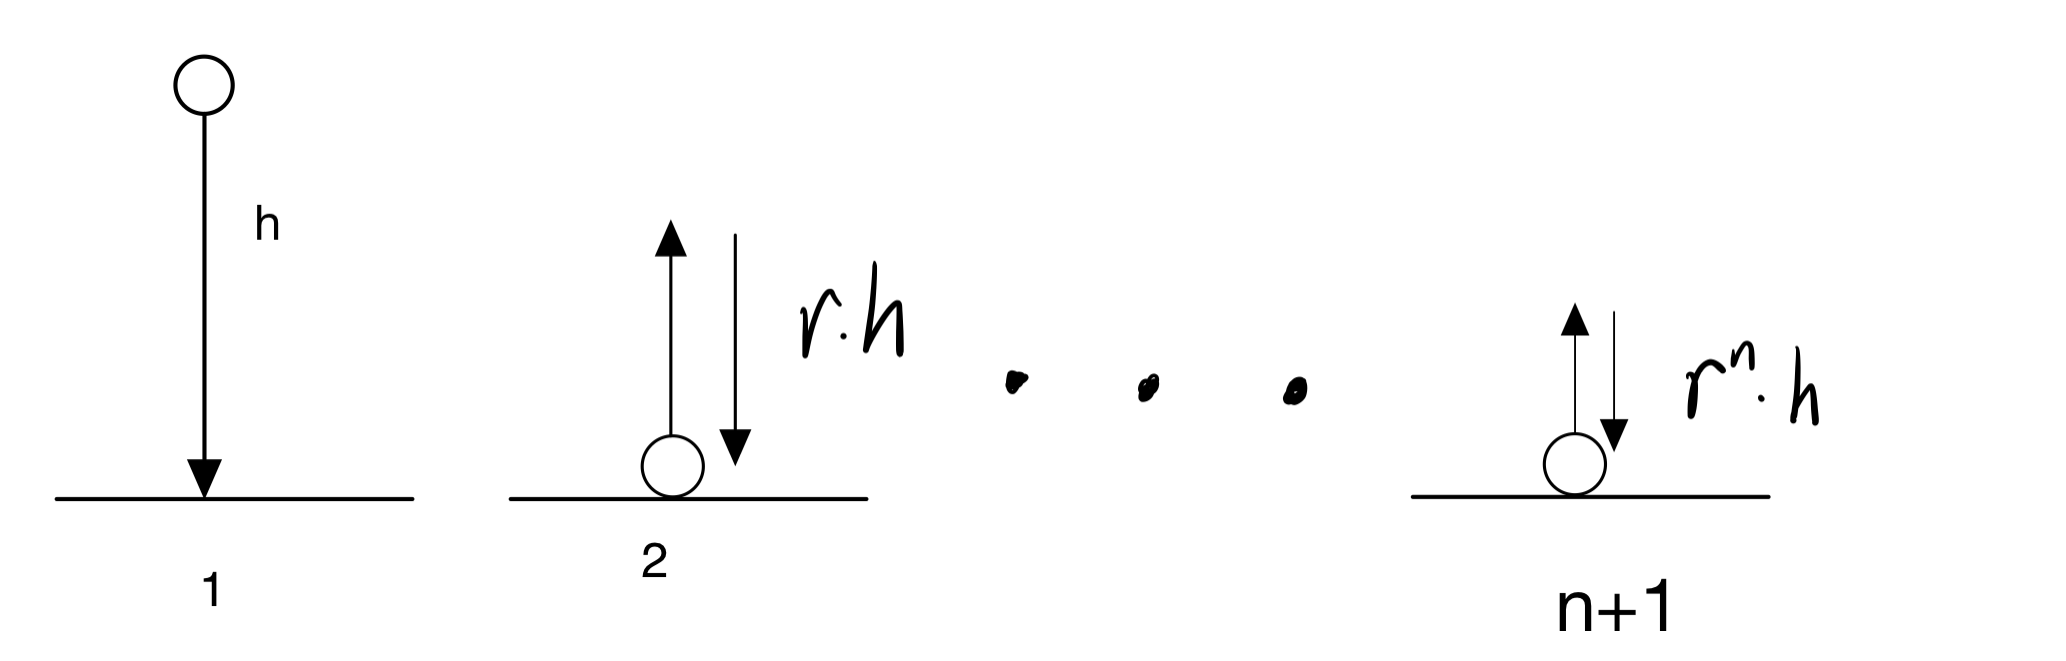
\includegraphics[scale=0.5]{Ex7.4.png}
    \caption{Figure 7.4}
    \end{figure}
The distance can be assessed through the image above (figure Ex7.4).
\par 
The first process : $h$
\par 
The second process : $2r\cdot h$
\par 
$. . .$
\par 
The $n$th process : $2r^{n-1}\cdot h$
\newline
Except for the first process is one-way, other process are all double-way
Thus, the total distance :
\begin{equation}
    \begin{aligned}
        D&=2(\sum_{n = 1}^{\infty} r^{n-1} \cdot h)-h\\
        &=\frac{2h}{1-r}-h
    \end{aligned}
    \end{equation}

\section{Ex7.5}
We can know from the question that 
$$\displaystyle \sum \frac{1}{n}= \sum _{n\in X} \frac{1}{n} +\sum _{n \in \mathbb{N}^* \backslash X} \frac{1}{n}$$
Because 
\begin{equation}
    \begin{aligned}
        \displaystyle \sum _{n \in \mathbb{N}^* \backslash X} \frac{1}{n} &=
        \frac{1}{9}+\frac{1}{81}+\dots+\frac{1}{9^k}+\dots\\
        &=\frac{1}{9}\sum \frac{1}{n}
    \end{aligned}
    \end{equation}
So, $\displaystyle \sum _{n \in \mathbb{N}^* \backslash X} \frac{1}{n}$ diverges.
\newline
Then, we can find that $\displaystyle\sum _{n\in X} \frac{1}{n}=\frac{8}{9}\sum \frac{1}{n}$
So, $\displaystyle \sum _{n \in X} \frac{1}{n}$ also diverges.


\section{Ex7.6}
\begin{figure}[H]
    \centering
    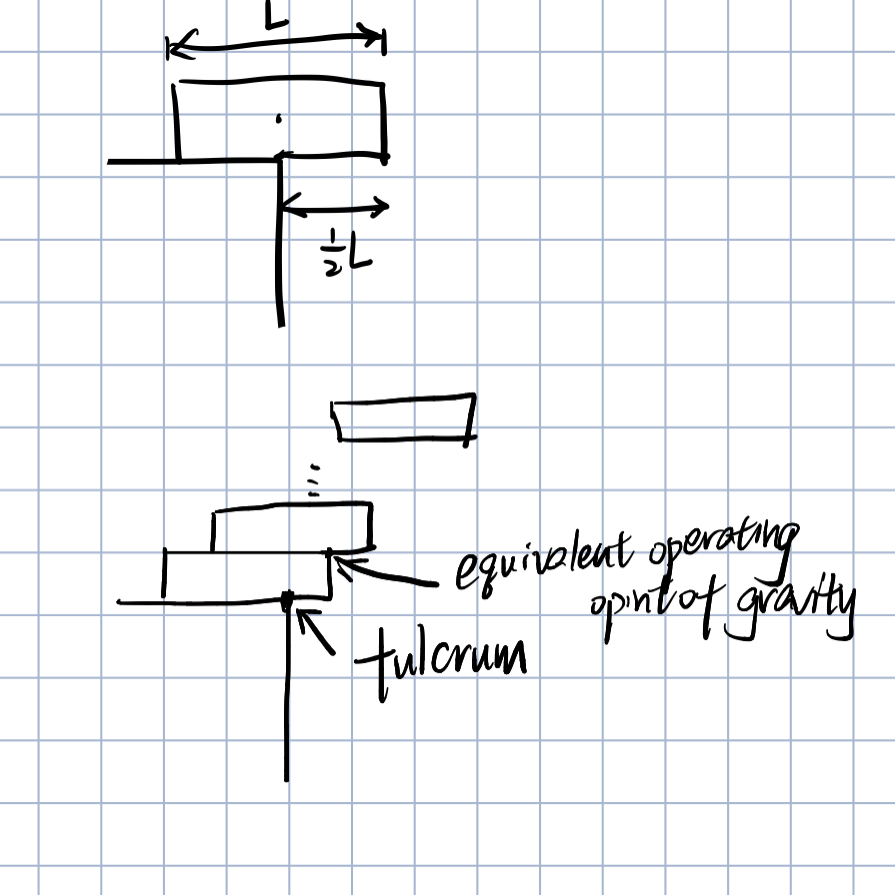
\includegraphics[scale=0.5]{Ex7.6.1.png}
    \caption{Figure 7.6.1}
    \end{figure}
We can model the question(figure 7.6.1). When there are $n+1$ bricks,
 assume that the mass of each brick is $m$, the acceleration 
 of gravity is $g$, the length of the lever is $L$ and the 
 distance between the middlepoint and the right end is 
 $l_{n+1}$. We can then simplify it into a lever (show in figure 7.6.2).
\begin{figure}[H]
    \centering
    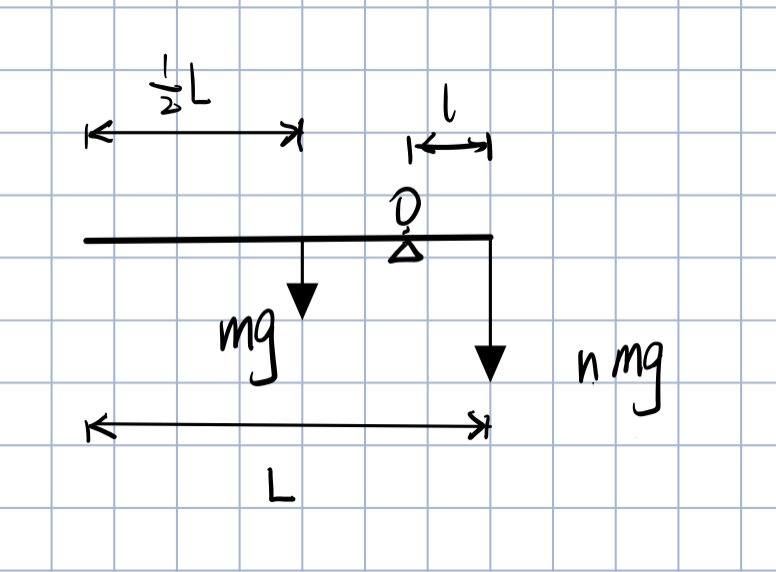
\includegraphics[scale=0.5]{Ex7.6.2.png}
    \caption{Figure 7.6.2}
    \end{figure}
    According to lever principle, we can know that 
\begin{equation}
    \begin{aligned}
        mg(\frac{L}{2}-l_{n+1})&=nmgl_{n+1}\\
        \frac{1}{2}mgL-mgl_{n+1}&=nmgl_{n+1}\\
        l_{n+1}&=\frac{L}{2(n+1)}\\
        l_{n+1}&=\frac{L}{2}\cdot\frac{1}{n+1}
    \end{aligned}
    \end{equation}
So we can know $\sum_{n = 1}^{\infty}l_{n+1} $ diverges. Thus, 
the tower can extend to infinite far.

\section{Ex7.7}
\subsection{7.7.1}
\begin{equation}
    \begin{aligned}
        \sum_{n = 1}^{\infty}  \frac{2^{2n}\cdot 3^{3n}}{5^{3n}}&=
        \sum_{n = 1}^{\infty} \frac{4^n 27^n}{125^n}\\
        &=(\frac{108}{125})^n\\
        &=\frac{108}{17}
    \end{aligned}
    \end{equation}
    So, we can know the $\displaystyle\sum_{n = 1}^{\infty}  \frac{2^{2n}\cdot 3^{3n}}{5^{3n}}$
    converges.
\subsection{7.7.2}
Because we know when $n>3$, $n^2-3n+1>0$
Thus, we can know:
\begin{equation}
    \begin{aligned}
        a_{n}:=\sum_{n = 1}^{\infty}  \frac{n+4}{n^2-3n+1}&=
        \sum_{n = 1}^{3}  \frac{n+4}{n^2-3n+1}+
        \sum_{n = 4}^{\infty}  \frac{n+4}{n^2-3n+1}\\
        &>\sum_{n = 1}^{3}  \frac{n+4}{n^2-3n+1}+
        \sum_{n = 4}^{\infty}  \frac{n+4}{n^2+16n+16}\\
        &=\sum_{n = 1}^{3}  \frac{n+4}{n^2-3n+1}+
        \sum_{n = 4}^{\infty}  \frac{1}{n+4}=:b_{n}
    \end{aligned}
    \end{equation}
Because $\displaystyle \sum_{n = 4}^{\infty}  \frac{1}{n+4}$ diverges, so $b_{n}$ diverges.
\newline
Thus $\displaystyle a_{n}=\sum_{n = 1}^{\infty}  \frac{n+4}{n^2-3n+1}$ diverges
as $0<b_{n}<a_{n}$.

\subsection{7.7.3}
Let $\displaystyle a_{n}:=\frac{n^4}{3^n}$. We will use deduction to 
prove that when $n \ge 32$, $n^4<2^n$.
\newline
Firstly, when $n=32$, $(32)^4=2^{20}<2^{32}$
\newline
Secondly, assume that when $n=k$,$n \in \mathbb{N}^*,k\ge 32$
, we also have $2^k>k^4$.
\newline
So, when $n=k+1$, because
$$\frac{(k+1)^4}{k^4}=(\frac{k+1}{k})^4<(\frac{33}{32})^4<2$$
Thus, 
$$2^{k+1}=2\cdot 2^{k}>2\cdot k^n >(k+1)^4$$
So, we have proved that when $n \ge 32$, $n^4<2^n$.
\newline
We get 
$$\sum_{n = 1}^{\infty} a_{n} =\sum_{n = 1}^{32} a_{n} 
+\sum_{n = 33}^{\infty}\frac{n^4}{3^n}
<\sum_{n = 1}^{32}a_{n}+
\sum_{n = 33}^{\infty} (\frac{2}{3})^n:=b_{n} $$
\newline
Because we know that $\displaystyle \sum_{n = 33}^{\infty} (\frac{2}{3})^n$
converges.
So, $b_{n}$ converges. Thus $a_{n}$ converges as $0<a_{n}<b_{n}$,

\subsection{7.7.4}
Let $\displaystyle a_{n}:=\frac{2^n}{n!}$, Then, 
$$\displaystyle 
\lim_{x \to \infty} \frac{a_{n+1}}{a_{n}}
=\lim_{x \to \infty}\frac{\frac{2^{n+1}}{(n+1)!}}{\frac{2^n}{n!}} 
=\lim_{x \to \infty} \frac{2}{n+1}=0$$
Thus,$\displaystyle a_{n}=\frac{2^n}{n!}$ converges.

\subsection{7.7.5}
Let $\displaystyle a_{n}:=\frac{2^n}{n^n}$. Then,
$$\displaystyle \lim_{x \to \infty} \frac{a_{n+1}}{a_{n}}
=\lim_{x \to \infty} \frac{2n^n}{(n+1)^(n+1)}
=\lim_{x \to \infty} 2\cdot(\frac{n}{n+1})^n \cdot (\frac{1}{n+1})
=0 $$
Thus, $\displaystyle a_{n}=\frac{2^n}{n^n}$ converges.

\subsection{7.7.6}
We can know from 
$\displaystyle \sum_{n = 1}^{\infty} \frac{n}{10n^3-100} $
that when $n>4$, $\displaystyle \sum_{n = 1}^{\infty} \frac{n}{10n^3-100}>0 $
\newline
And then, we will prove that when $n>4$, $\displaystyle \frac{n}{10n^3-100}>0 $
strictly decreases.
\par
Proof:\newline
For $\forall n>4$ , 
\begin{equation}
    \begin{aligned}
        \frac{n+1}{10(n+1)^3-100}-\frac{n}{10n^3-100}
        &=\frac{1}{10}(\frac{n+1}{(n+1)^3-10}-\frac{1}{10}(\frac{n}{n^3-10}) \\
        &=\frac{1}{10}\cdot\frac{-2n^3-3n^2-n-10}{[(n+1)^3-10](n^3-10)}<0
    \end{aligned}
    \end{equation}
Thus, $\displaystyle \frac{n}{10n^3-100}>0 $ strictly decreases.\newline
Then, we will prove $a_{n}:=\sum_{n = 1}^{k}\displaystyle \frac{n}{10n^3-100}$ is Cauchy squence.
\par
Proof:\newline
For all $n>4$ and fixed $p$, 
\begin{equation}
    \begin{aligned}
        \sum_{n = 1}^{k+p} \frac{n}{10n^3-100}-\sum_{n = 1}^{k} \frac{n}{10n^3-100}
        =\sum_{n = k+1}^{k+p} \frac{n}{10n^3-100}
    \end{aligned}
    \end{equation}

Because 
\begin{equation}
    \begin{aligned}
        \left|\sum_{n = k+1}^{k+p} \frac{n}{10n^3-100}-\sum_{n = k+2}^{k+p+1} \frac{n}{10n^3-100}\right|
        &=\frac{k+p+1}{10(k+p+1)^3-100}-\frac{k+1}{10(k+1)^3-100} \\
        &<\frac{p}{10(k+1)^3-100}
    \end{aligned}
    \end{equation}
    We can know that $\displaystyle \lim_{k \to \infty} \frac{p}{10(k+1)^3-100} =0$. So 
    $\forall \varepsilon>0,\exists k \in \mathbb{N}^*$, there exists $\varepsilon$ that satisfies
    $$\left|\sum_{n = 1}^{k+p} \frac{n}{10n^3-100}-\sum_{n = 1}^{k} \frac{n}{10n^3-100}\right|<\varepsilon$$
    We have prove $a_{n}:=\sum_{n = 1}^{k} \displaystyle \frac{n}{10n^3-100}$ is Cauchy squence.
    And then we can know $\displaystyle \sum_{n = 1}^{\infty} \frac{n}{10n^3-100} $ converges.
\end{document}
